\section{Tensegrity domes}
We will now consider the situation with added bars, but still using the constraint of fixed nodes. Our new optimisation problem has the following objective function:
\begin{equation}
\begin{aligned}
    \label{energy}
    &E(X) = \sumset{B}\big(\ebe + \ebg\big) + \sumset{C} \ece + \ee \\
    & \text{such that } x^{(i)} = p^{(i)}, i=1,...,M
\end{aligned}
\end{equation}

which still leaves us with a free optimization problem. However, the situation will be slightly more complicated.

The objective function \eqref{energy} is not generally differentiable. We see that the elastic energy model for bars is the same as cables for $\xnorm > \el$ with a different constant $k$, which gives us similar partial derivatives:
\begin{equation*}
\delx \ebe = \frac{c}{\el^2} (1- \frac{\el}{\xnorm}) (x_k^{(i)} - x_k^{(j)})
\end{equation*}

\textbf{fix uttrykket over}
Note that this expression is valid for all values of $\xnorm$, which means that the function is not differentiable when $\xnorm = 0$. However, the distance being $0$ would imply two nodes being in the same position which will clearly never happen in practice, so this is not a problem. That being said, the fact that our function has such little smoothness causes us some other problems.

\subsection{Optimality conditions for tensegrity domes}
For $C^2$ optimization problems, the general necessary optimality conditions for a solution $X^*$ is

\begin{align*}
    &\nabla E(X^*) = 0\\
    & H_f(X^*) \text{ is positive semi-definite}
\end{align*}
Unfortunately our objective function is not $C^2$ - it's not even $C^1$ strictly speaking. For all practical purposes we have the necessary condition $\nabla E(X^*) = 0$, as long as all nodes have unique positions, but we have no neccesary second order conditions.

Similarly, the typical sufficient condition of $H_f(X^*)$ being positive definite is not applicable. For convex functions, the one condition we actually do have of $\nabla E(X)=0$ would be sufficient. However it turns out that our objective function is no longer convex.

\textbf{Spørsmål:} 
Teorem: 
f er convex hvis og bare hvis $H_f(x)$ er positive demi-definite for alle x.

Teorem: Nabla x = 0 er godt nok for konvekse funksjoner til å gi minimizer. 

-Men generelt må vi jo ha positive definiteness, ikke semi-definiteness? Får ikke helt dette til å stemme..

\subsection{Non-convexity}
In order for a function to be convex we need it to hold for all $X,Y \in \mathbb{R}^{3N}$ and any $0\leq \lambda \leq 1$ Therefore, we will consider $\lambda = \frac{1}{2}$, and $X,Y$ such that 
\begin{equation*}
    \rVert x^{(i)}-x^{(j)} \lVert, \rVert y^{(i)}-y^{(j)} \lVert < \el \quad \forall \quad i,j \in N
\end{equation*}
Now let $Y = -X$, that is: $\xx = -(y^{(i)}-y^{(j)}) = y^{(j)}-y^{(i)}$ such that
\begin{equation}
    \label{energyConv1}
    E^{cable}_{elast}(\lambda X + (1-\lambda) Y) = E^{cable}_{elast}(\frac{1}{2}X + \frac{1}{2}(-X)) = E^{cable}_{elast}(0) = \sumset{E} \frac{c}{2 \el^2} ( \rVert 0 \lVert - \el)^2 = \sumset{E}\frac{c}{2}
\end{equation}
On the other hand, we have
\begin{equation}
\label{energyConv2}
\begin{aligned}    
    &\lambda E^{cable}_{elast}(X) + (1-\lambda)E^{cable}_{elast}(Y) \\&= \frac{1}{2}E^{cable}_{elast}(X) + \frac{1}{2}E^{cable}_{elast}(-X) \\& 
    = \frac{1}{2}\sumset{E} \frac{c}{2\el^2} (\xnorm - \el)^2 + \frac{1}{2} \sumset{E}\frac{c}{2\el^2} (\rVert-(\xx)\lVert)^2\\
    &= \sumset{E}\frac{c}{2\el^2}(\rVert(\xx)\lVert - \el )^2= \sumset{E}\frac{c}{2\el^2} (\xnorm^2 - 2\xnorm \el + \el^2) \\
    &=\sumset{E}\frac{c}{2\el^2} \xnorm (\xnorm - 2 \el) + \sumset{E}\frac{c}{2\el^2}\el^2
    \end{aligned}
\end{equation}

In order for the function to be convex we need the difference between the two expressions to be non-negative:
\begin{equation}
    =\sumset{E}\frac{c}{2\el^2} \xnorm (\xnorm - 2 \el) \geq 0
\end{equation}
We see that the expression is only convex if we have
$$\xnorm \geq 2 \cdot \underset{{e_{ij} \in \mathcal{E}}}{\text{min}}\el$$
which means that the expression is only convex when the bars are more than twice the length of the shortest bar. Thus, the objective function is not convex. $\square$
\textbf{men her har vi en condition på konveksitet da, kan det brukes til noe?}

The fact that the function is non-convex means that we need the general optimality conditions, as well as restricting our choice of algorithms. It also means that we have local minima that are not global, as seen in figure \ref{fig:local_optimizer}:

Fix a node $p^{(1)}$, and consider a free node $x^{(2)}$ that is placed at least a distance $l_{12}$ above the $p^{(1)}$. At this starting position the bar will not have any elastic energy, so the gravity will bring the node downwards until the gravity is equally strong as the elastic force from the bar, which will be a local minima. However, it will not be a global minima as we will have lower energy if we instead placed $x^{(2)}$ below $p^{(1)}$ as seen in the rightmost drawing. 

\begin{figure}
    \centering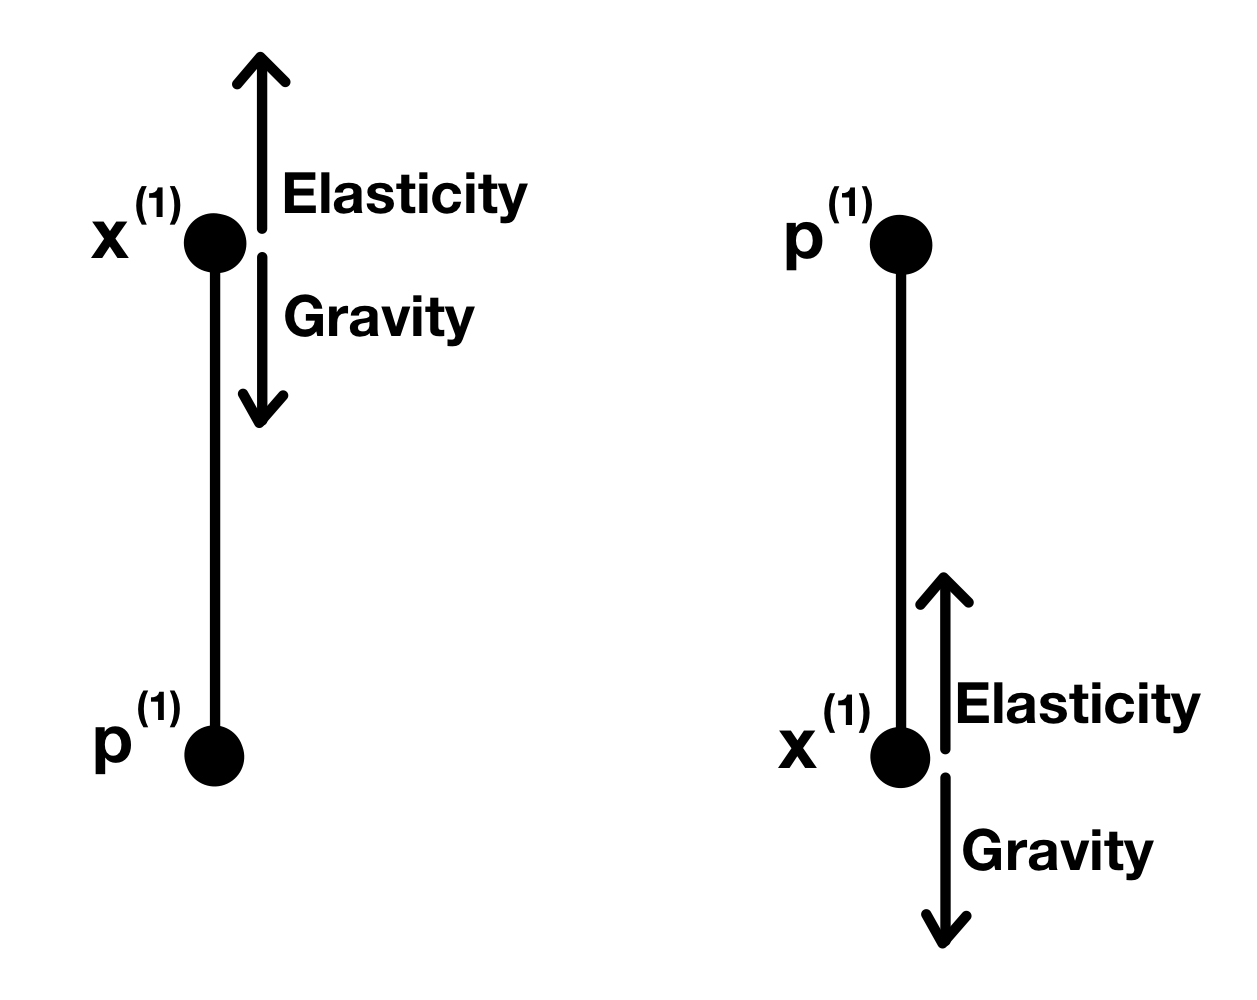
\includegraphics[width=0.5\columnwidth]{Bilder/local_optimizer.jpeg}
    \caption{Local optimizer to the left, global optimizer to the right.A bar is connected between the fixed node $p^{(1)}$, and free node $x^{(2)}$.}
    \label{fig:local_optimizer}
\end{figure}

We see that we have an equillibrium in the first case where the elasticity is equal to the gravity.

\section{Tensegrity domes in constrained optimization}
We will now consider the full problem \eqref{energy} with the constraints given by 
\begin{equation}
    x_3^{(i)} \geq 0 \quad \forall \quad i = 1,...,N
\end{equation}

As this is a constrained optimization problem, we will the Lagrangian \begin{equation}
    \mathcal{L}(X,\lambda) = E(X) - \sum_{i \in \ \mathcal{I}}\lambda_i c_i(x^{(i)})
\end{equation}
Where $c_i(x) = x^{(i)}_3$.

The first order optimality conditions for a given $(X^*,\lambda^*)$ are \begin{equation}
\begin{aligned}
       &\nabla_x \mathcal{L}(X,\lambda^*)=0\\ 
       &x^{*(i)}_3 \geq 0,\quad i = 1,...,N\\
       &\lambda_i^* \geq 0 ,\quad i = 1,...,N\\
       & \lambda_i^* x^{*(i)}_3 = 0,\quad i = 1,...,N
\end{aligned}
\end{equation}

LICQ: $\nabla x_3^{(i)} = \frac{\partial}{\partial_{x_3}} x_3^{(i)} =(,..., 1,...,0) \forall i$, so we have LICQ.

Therefore the KKT conditions are neccesary.

They are not sufficient as our problem is not convex.